\documentclass[table,dvipsnames,11pt,a4paper]{article}

\usepackage[utf8]{inputenc}
\usepackage{lmodern}
\usepackage{textcomp}
\usepackage{float}
\usepackage{tikz}
\usepackage[top=80pt,bottom=120pt,left=75pt,right=75pt]{geometry}
\usepackage{microtype}
\usepackage{graphicx}
\usepackage{listings}
\usepackage{subcaption}
\usepackage{parskip}
\usepackage{appendix}
\usepackage{bm}
\usepackage{amsmath}
\usepackage{amssymb}
\usepackage{xcolor}
\usepackage{relsize}
\usepackage{enumitem}
\usepackage{amsfonts}
\usepackage{textgreek}
\usepackage{booktabs}
\usepackage{array}
\usepackage{xfrac}
\usepackage[labelfont=bf,font=footnotesize]{caption}
\usepackage[hypertexnames=false,hidelinks]{hyperref}
\usepackage[noabbrev,nameinlink,capitalize,poorman]{cleveref}

\bibliographystyle{unsrt}

% \renewcommand{\thesection}{Task \arabic{section}}
\renewcommand{\thesubsection}{\arabic{subsection}}

\newcommand{\argmax}{\text{argmax}}
\newcommand{\rand}{\text{rand}}

\newcommand{\appendixA}{\hyperref[param_sweep_result_appendix]{Appendix A}}

\usetikzlibrary{matrix}
\usetikzlibrary{fit}
\usetikzlibrary{plotmarks}
\usetikzlibrary{positioning}
\usetikzlibrary{external}
\tikzexternalize[prefix=tikz/]

\setcounter{topnumber}{10}
\setcounter{bottomnumber}{10}
\setcounter{totalnumber}{10}
% \renewcommand{\floatpagefraction}{1}

\definecolor{coolgray}{rgb}{0.95,0.95,0.95}
\lstset{
	language=Python,
	backgroundcolor=\color{coolgray},
	tabsize=2,
	keywordstyle=\bfseries\color{OliveGreen},
	numbers=left,
	breakatwhitespace=true,
	captionpos=t,
	frame=single,
	basicstyle=\ttfamily\tiny,
	extendedchars=true,
	emphstyle=\color{Blue},
	showstringspaces=false,
	morekeywords={with, as},
	literate={✗}{X}1 {●}{o}1 {×}{$\times$}1 {→}{\textrightarrow}1 {↓}{\textdownarrow}1 {←}{\textleftarrow}1 {↑}{\textuparrow}1 {¡}{ }1,
}


\begin{document}

\begin{titlepage}
	\centering
	\includegraphics[width=\textwidth]{City\_logo} \\[4em]
	\begin{bfseries}
		\begin{Huge}
			Deep Reinforcement Learning \\[35pt]
			\textsl{Written Report}
		\end{Huge}
	\end{bfseries}
	\vfill{}
	\begin{large}
		\textbf{Github repo} & \url{https://github.com/mfixman/ai-reinforcement} \\[1em]
	\end{large}
	\begin{LARGE}
		\begin{sffamily}
			Martin Fixman and Sean Lim \\
			and Sean Lim and Martin Fixman \\
			2023/2024 Term \\
                Github Link: https://github.com/mfixman/ai-reinforcement \\
		\end{sffamily}
	\end{LARGE}
\end{titlepage}

\renewcommand{\thesection}{Basic Task}

\newcommand{\upa}{\mathlarger{\uparrow}}
\newcommand{\downa}{\mathlarger{\downarrow}}
\newcommand{\lefta}{\mathlarger{\leftarrow}}
\newcommand{\righta}{\mathlarger{\rightarrow}}

\section{Q Learning}

\subsection{Working Environment}

\begin{figure}[h]
	\begin{subfigure}{.49\textwidth}
		\centering
		\includegraphics[width=170pt,height=125pt]{snow_original.png}
		\caption{Original puzzle}
	\end{subfigure}
	\begin{subfigure}{.49\textwidth}
		\centering
		\includegraphics[height=125pt]{snow_2.png}
		\caption{Puzzle solution}
	\end{subfigure}
	\caption{An example of a Pokémon Ice puzzle}
	\label{large_map}
\end{figure}

In this task we present a solver of \emph{Pokémon Ice Puzzles}, a kind of ice puzzle where the player starts at a certain position $s$ and has the objective to reach its objective $e$ in as few steps as possible.

At each turn, the player can do one of four movements: $\{\upa, \downa, \lefta, \righta\}$.
As the environment is ice, when the user walks in any direction is slips on the ice and keeps going on the same direction until hitting a rock or the edge.

The problem statement for the agent is simple: Arrive at the end goal in the least amount of steps possible. The agent would need to know which action constitutes to the next state that leads it closer to the end point.

\newcommand{\coor}[2]{\left\langle #1, #2 \right\rangle}
\newcommand{\yx}{\coor{y}{x}}
\newcommand{\obs}{\mathcal{O}}
\newcommand{\state}{\mathcal{S}}
\newcommand{\reward}{\mathcal{R}}

\subsection{State Transition and Reward Functions}
The state function $\state$, along with the transition and reward functions $\mathcal{T}$ and $\reward$ can be defined as the following, where $\obs_{\yx}$ is true if and only if there is an obstacle on position $\yx$.
\begin{gather*}
	\state = \yx \qquad \mathcal{D} \in \left\{ \upa, \downa, \lefta, \righta \right\} \\
	\begin{aligned}
		&T_{\yx}\left(\upa\right) &= \coor{t + 1}{x} &&&\text{where } \obs_{\coor{t}{x}} \wedge \neg \obs_{\coor{q}{x}} \forall q \in \left(t, y\right) \\
		&T_{\yx}\left(\downa\right) &= \coor{t - 1}{x} &&&\text{where } \obs_{\coor{t}{x}} \wedge \neg \obs_{\coor{q}{x}} \forall q \in \left(y, t\right) \\
		&T_{\yx}\left(\lefta\right) &= \coor{y}{t + 1} &&&\text{where } \obs_{\coor{y}{t}} \wedge \neg \obs_{\coor{y}{q}} \forall q \in \left(t, x\right) \\
		&T_{\yx}\left(\righta\right) &= \coor{y}{t - 1} &&&\text{where } \obs_{\coor{y}{t}} \wedge \neg \obs_{\coor{y}{q}} \forall q \in \left(x, y\right)
	\end{aligned} \\
	\reward(\yx) = \begin{cases}
		100 & \text{if } e = \yx \\
		0 & \text{otherwise}
	\end{cases}
\end{gather*}

In simpler terms, each action the agent makes at a certain point relocates the agent to the last viable open space which is not blocked by the edges of the map or any obstacles. Hence, the states are defined by all the spots that are not occupied by the obstacles or are not edges, while the action space are of the 4 directional functions. It is important to note here that the number of avaiable states are not all squares that are not obstacles or edges, but rather only a select few spaces where the agent can step on when it bumps into the obstacles or edges.

\subsection{Q Function and parameters}

This transition function allows us to define an iterative $Q$ function, which should be used to find the objective $Q^\pi$ function.
\begin{gather*}
	s \in \mathcal{S} \qquad a \in \mathcal{D} \\
	Q^{k + 1}(s, a) = \alpha \cdot \left( \reward( T( a, s ) ) + \gamma \cdot \max{Q^k(s, a)} \right) - Q^k(s, a)
\end{gather*}

The probability next action $a$ is defined depending on the policy used, where $\pi^k(a \mid s)$ represents the probability of choosing action $a$ with state $s$ at point $k$. The variables $\alpha$ and $\gamma$ represent the learning rate and the discount rate respectively, where the former addresses how much the agent learns per step, while the latter defines how much the agent places significance on the current rewards or future rewards.
\begin{gather*}
	\intertext{\textbf{\textepsilon-Greedy Policy}: choose the best policy with probability $\varepsilon$, randomly otherwise.}
	\pi^k(a \mid s) = 
		(1 - \varepsilon) \cdot \frac{1}{\mathcal{D}} + \varepsilon \cdot \begin{cases}
			1 & \text{if } a = \argmax_{a'} (Q^k(s, a')) \\
			0 & \text{otherwise}
		\end{cases} \\
	\intertext{\textbf{Boltzmann Policy}: choose policy using the softmax of the Q-value}
	\pi^k(a \mid s) = \frac{e^{Q^k(s, a)}}{\sum_{a' \in \mathcal{D}}{e^{Q^k(s, a')}}}
\end{gather*}

The epsilon greedy policy starts exploring the environment followed by exploiting, where the agent begins to use the knowledge gained from exploring and derive the best values it sees fit to carry out the actions that gives it the best rewards based on that knowledge. In that sense, the epsilon greedy policy is more deterministic compared to the Boltzmann policy, which also utilises exploration and exploitation, but during exploitation, rather than carrying out the best values it has learnt through exploration, the Boltzmann policy instead chooses an action with probability derived from the equation above. Because of this, the Epsilon-greedy policy is more likely to converge, while the Boltzmann policy is more likely to make more informed actions in cases where two actions in the current time yield marginally different results, leading to more adaptability in more complex environments.

\subsection{Parameter sweep}
\label{param_sweep}
To find the best parameters, we run a parameter sweep on the map in \cref{large_map} for each combination of parameters in \cref{param_sweep_params}; this map is large enough to make it suitable for a parameter sweep.

\begin{table}[h]
	\scriptsize
	\centering
	\begin{tabular}{>{\bfseries}r | l l l l}
		\toprule
		Hyperparameter & \multicolumn{4}{c}{Values} \\
		\midrule
		Policy & \multicolumn{4}{l}{\begin{tabular}{l l}$\varepsilon$-Greedy & Boltzmann\end{tabular}} \\
		$\alpha$ & 0.1 & 0.5 & 0.7 & 0.9 \\
		$\gamma$ & 0.9 & 0.99 && \\
		$\varepsilon$ Decay Rate & 0.75 & 0.9 & 0.99 & \\
		\bottomrule
	\end{tabular}
	\caption{The parameter sweep considered every possible combination of these parameters.}
	\label{param_sweep_params}
\end{table}

Each combination was run 10 times until the Q matrix converged to a precision of $10^{-12}$ and results were averaged.
The final results, which contain the best parameters, can be found in \appendixA{}
Some interesting results can be found in \cref{param_sweep_interesting}.

\begin{table}[h]
	\scriptsize
	\centering
	\begin{tabular}{>{\bfseries}r r l r | r r r r}
		\toprule
		Policy & $\alpha$ & $\gamma$ & $\varepsilon$ Decay &
		E.\ to Conv & Best route & E.\ to Done & E.\ to Best \\
		\midrule
		\rowcolor{YellowGreen}
		\textepsilon{}-Greedy & 0.5  & 0.90  & 0.99 & 139 & 16.00 & 31.80  & 97 \\
		\textepsilon{}-Greedy & 0.9 & 0.90  & 0.90 & 51  & 16.80 & 12.00  & 26 \\
		\midrule
		Boltzmann & 0.2 & 0.90 & 0.75 & 666  & 16.20 &  82.70 &  224 \\
		Boltzmann & 0.9 & 0.90 & 0.99 & 126  & 17.40 &  37.30 &   86 \\
		Boltzmann & 0.7 & 0.90 & 0.75 & 205  & 17.60 &  48.70 &   58 \\
		\bottomrule
	\end{tabular}
	\caption{Some notable results taken from \appendixA{}.}
	\label{param_sweep_interesting}
\end{table}

We can observe the following.
% \begin{itemize}
% 	\item The \textepsilon{}-Greedy policy converges faster and produces a significantly better result.
% 	\item Generally having high $\varepsilon$ Decay represents better results.
% 	\item There is a significant correlation between convergence speed and how good the solutions are.
% \end{itemize}
\subsubsection{Difference in Policies}
The Epsilon-Greedy policy converges faster, as expected from the hypothesis defined above as the Epsilon-Greedy policy is more deterministic as the agent will always take the actions that contain the highest Q-values.  In this sense, the Epsilon-Greedy policy performs better in the ideal scenario that the agent is able to completely learn the environment, meanwhile the Boltzmann policy outperforms the Epsilon-Greedy policy as seen in cases where the agent begins exploiting too early due to low epsilon decay factor, in which case the Boltzmann policy is able to derive a better solution than the Epsilon-Greedy policy as it still considers actions which yield marginally different rewards.

\subsubsection{Difference in epsilon decay factor}
Furthermore, a lower epsilon decay factor generally leads to quicker convergence speeds. This is expected as the epsilon decay factor directly impacts how quickly the agent transitions from exploring to exploiting. 

For most cases, the agent was never able to determine the best route retrospectively (16) as the agent often has already begun exploiting before the agent fully learns the environment provided. This is especially true with epsilon-greedy policies as explained above. 

\subsubsection{Convergence speed vs Solution quality}
Another observation can be made on the tradeoff between the convergence speed and the quality of the solutions, where lower convergence speed allows the agent to learn the environment more and achieve an optimal solution, while a faster convergence speed prompts better training time at the cost of poorer quality solutions.

\subsubsection{Difference in Alphas}
Besides that, a larger alpha directly impacts how much the agent takes the learning in that timestep into account. Excessively large alpha values generally do not perform well as the agent often overestimates the Q-values, leading to the agent to overfit towards certain actions that provide rewards in the first few episodes, causing the agent to be unable to optimize the solution in the environment as the agent already thinks it is doing the best solution. Similarly, excessively low alpha values cause the agent to struggle to find the best solutions locally in a reasonable timeframe. In cases where epsilon decay is low, the agent takes over 400 episodes in both policies to achieve what it believes to be the best result.

\subsection{Analysing this solution}
We choose the parameter combination that converges the fastest between the ones that \emph{always} found the best solution; that's marked in \colorbox{YellowGreen}{green} in table \ref{param_sweep_interesting}

The solution found in \cref{param_sweep} takes on average 139 epochs to converge.
Of those, it takes an average of 31.8 epochs to find a solution, and 97 epochs to find \emph{the best} solution.
Despite taking significantly longer to converge due to its low learning rate, it always finds the optimal solution.

\begin{figure}[H]
	\centering
	\includegraphics[width=\textwidth]{task1_best_solution_by_epoch.png} \\[1ex]
	\includegraphics[width=\textwidth]{task1_qmatrix_convergence.png}
	\caption{Best solution found at each epoch and convergence of the Q-matrix of candidate solution and a few others. We can see that the high Epsilon-decay and low learning rate of our chosen solution make it both \emph{a solution} and \emph{the best solution} faster. Additionally, the best solution converges to a much larger mean Q value.}
\end{figure}

\vspace{-13pt}

\renewcommand{\textuparrow}{\ensuremath{\upa{}}}
\renewcommand{\textdownarrow}{\ensuremath{\downa{}}}
\renewcommand{\textleftarrow}{\ensuremath{\lefta{}}}
\renewcommand{\textrightarrow}{\ensuremath{\righta{}}}
\begin{figure}[H]
	\centering
	\begin{subfigure}{.42\textwidth}
		% \resizebox{\textwidth}{!}{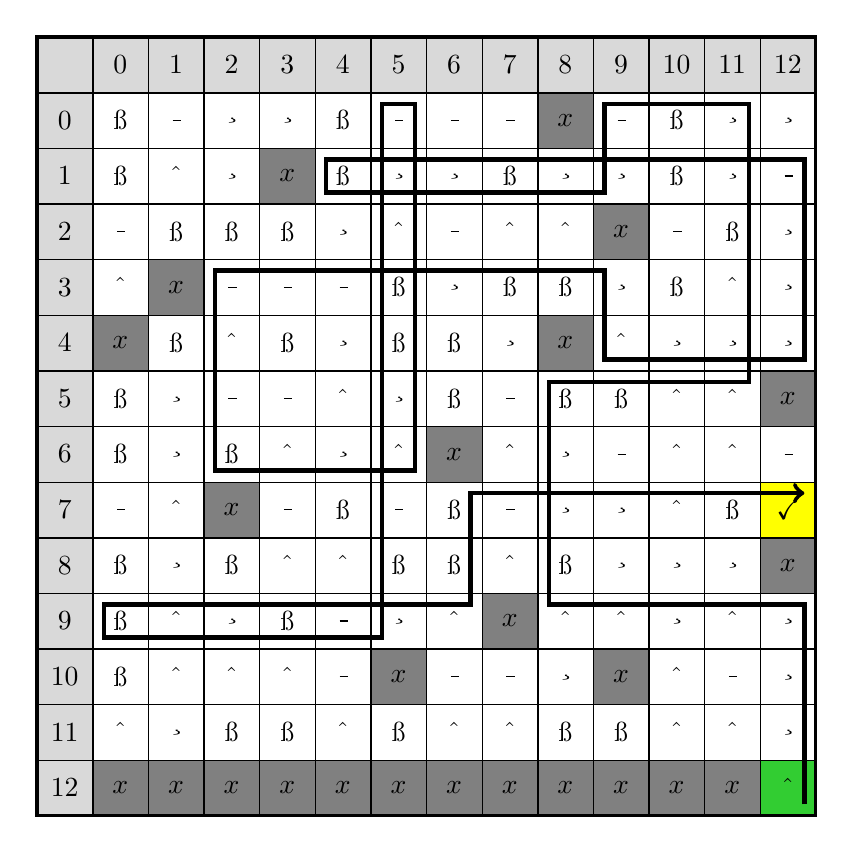
\begin{tikzpicture}[every node/.style={anchor=center}]
	\matrix (table) [
		matrix of nodes,
		nodes={draw, minimum height=20pt, minimum width=20pt, anchor=center, line width=.1pt},
		nodes in empty cells,
		execute at begin node = $,
		execute at end node = $,
		column 1/.style={nodes={fill=gray!30, execute at begin node=$, execute at end node=$}},
		row 1/.style={nodes={fill=gray!30, execute at begin node=$, execute at end node=$}}
	]{
   & 0 & 1 & 2 & 3 & 4 & 5 & 6 & 7 & 8 & 9 & 10 & 11 & 12 \\
 0 & → & ↓ & ← & ← & → & ↓ & ↓ & ↓ & |[fill=Gray]| x & ↓ & → & ← & ← \\
 1 & → & ↑ & ← & |[fill=Gray]| x & → & ← & ← & → & ← & ← & → & ← & ↓ \\
 2 & ↓ & → & → & → & ← & ↑ & ↓ & ↑ & ↑ & |[fill=Gray]| x & ↓ & → & ← \\
 3 & ↑ & |[fill=Gray]| x & ↓ & ↓ & ↓ & → & ← & → & → & ← & → & ↑ & ← \\
 4 & |[fill=Gray]| x & → & ↑ & → & ← & → & → & ← & |[fill=Gray]| x & ↑ & ← & ← & ← \\
 5 & → & ← & ↓ & ↓ & ↑ & ← & → & ↓ & → & → & ↑ & ↑ & |[fill=Gray]| x \\
 6 & → & ← & → & ↑ & ← & ↑ & |[fill=Gray]| x & ↑ & ← & ↓ & ↑ & ↑ & ↓ \\
 7 & ↓ & ↑ & |[fill=Gray]| x & ↓ & → & ↓ & → & ↓ & ← & ← & ↑ & → & |[fill=Yellow]| \checkmark{} \\
 8 & → & ← & → & ↑ & ↑ & → & → & ↑ & → & ← & ← & ← & |[fill=Gray]| x \\
 9 & → & ↑ & ← & → & ↓ & ← & ↑ & |[fill=Gray]| x & ↑ & ↑ & ← & ↑ & ← \\
10 & → & ↑ & ↑ & ↑ & ↓ & |[fill=Gray]| x & ↓ & ↓ & ← & |[fill=Gray]| x & ↑ & ↓ & ← \\
11 & ↑ & ← & → & → & ↑ & → & ↑ & ↑ & → & → & ↑ & ↑ & ← \\
12 & |[fill=Gray]| x & |[fill=Gray]| x & |[fill=Gray]| x & |[fill=Gray]| x & |[fill=Gray]| x & |[fill=Gray]| x & |[fill=Gray]| x & |[fill=Gray]| x & |[fill=Gray]| x & |[fill=Gray]| x & |[fill=Gray]| x & |[fill=Gray]| x & |[fill=LimeGreen]|↑ \\
	};

	\foreach \row in {2,...,14} {
		\foreach \col in {2,...,14} {
			\pgfmathtruncatemacro{\rown}{\row - 2} % Adjust row number
			\pgfmathtruncatemacro{\coln}{\col - 2} % Adjust column number
			\node (c-\rown-\coln) at (table-\row-\col) {};

			\edef\cellname{c-\rown-\coln}
			\foreach \dir/\dx/\dy in {u/0/6pt, d/0/-6pt, l/-6pt/0, r/6pt/0, 
									  ul/-6pt/6pt, ur/6pt/6pt, 
									  dl/-6pt/-6pt, dr/6pt/-6pt} {
				\path (\cellname.center) ++(\dx, \dy) node (\cellname\dir) {};
			}
		}
	}
	\node[fit=(table-1-1)(table-14-14), draw, very thick, inner sep=0pt] {};

\draw [->, ultra thick]
(c-12-12dr.center) -- (c-9-12ur.center) -- (c-9-8ul.center) -- (c-5-8ul.center) -- (c-5-11ur.center) -- (c-0-11ur.center) -- (c-0-9ul.center) -- (c-1-9dl.center) -- (c-1-4dl.center) -- (c-1-4ul.center) -- (c-1-12ur.center) -- (c-4-12dr.center) -- (c-4-9dl.center) -- (c-3-9ul.center) -- (c-3-2ul.center) -- (c-6-2dl.center) -- (c-6-5dr.center) -- (c-0-5ur.center) -- (c-0-5ul.center) -- (c-9-5dl.center) -- (c-9-0dl.center) -- (c-9-0ul.center) -- (c-9-6ur.center) -- (c-7-6ur.center) -- (c-7-12ur.center);


\end{tikzpicture}

}
		\caption{After 23 epochs, with a path of length 24.}
	\end{subfigure}
	\begin{subfigure}{.42\textwidth}
		% \resizebox{\textwidth}{!}{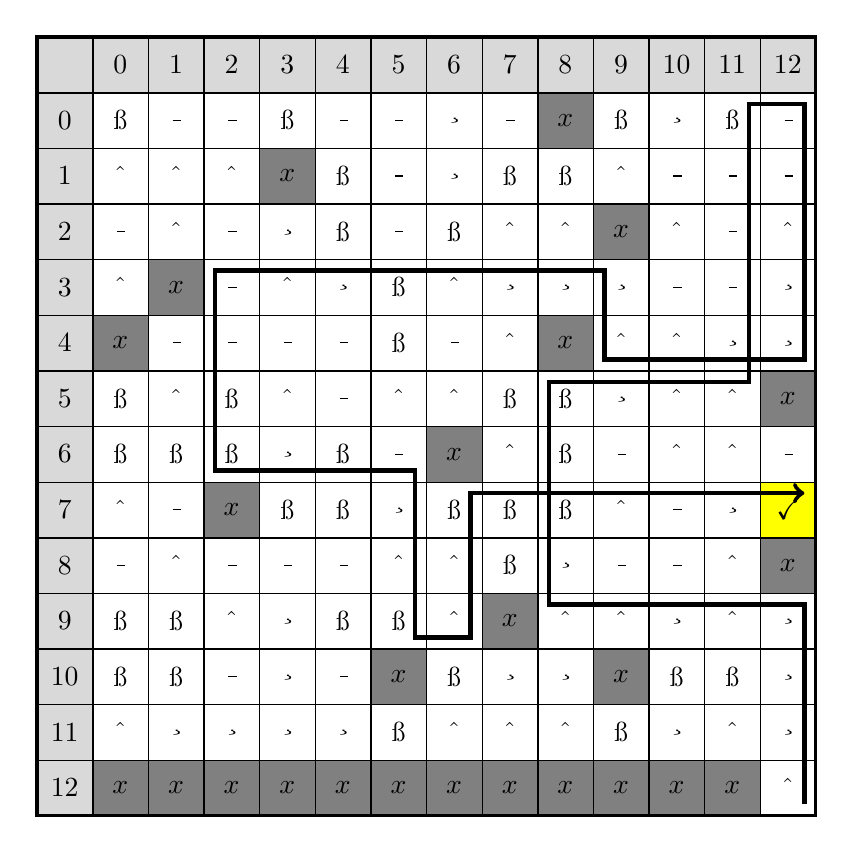
\begin{tikzpicture}[every node/.style={anchor=center}]
	\matrix (table) [
		matrix of nodes,
		nodes={draw, minimum height=20pt, minimum width=20pt, anchor=center, line width=.1pt},
		nodes in empty cells,
		execute at begin node = $,
		execute at end node = $,
		column 1/.style={nodes={fill=gray!30, execute at begin node=$, execute at end node=$}},
		row 1/.style={nodes={fill=gray!30, execute at begin node=$, execute at end node=$}}
	]{
   & 0 & 1 & 2 & 3 & 4 & 5 & 6 & 7 & 8 & 9 & 10 & 11 & 12 \\
 0 & → & ↓ & ↓ & → & ↓ & ↓ & ← & ↓ & |[fill=Gray]| x & → & ← & → & ↓ \\
 1 & ↑ & ↑ & ↑ & |[fill=Gray]| x & → & ↓ & ← & → & → & ↑ & ↓ & ↓ & ↓ \\
 2 & ↓ & ↑ & ↓ & ← & → & ↓ & → & ↑ & ↑ & |[fill=Gray]| x & ↑ & ↓ & ↑ \\
 3 & ↑ & |[fill=Gray]| x & ↓ & ↑ & ← & → & ↑ & ← & ← & ← & ↓ & ↓ & ← \\
 4 & |[fill=Gray]| x & ↓ & ↓ & ↓ & ↓ & → & ↓ & ↑ & |[fill=Gray]| x & ↑ & ↑ & ← & ← \\
 5 & → & ↑ & → & ↑ & ↓ & ↑ & ↑ & → & → & ← & ↑ & ↑ & |[fill=Gray]| x \\
 6 & → & → & → & ← & → & ↓ & |[fill=Gray]| x & ↑ & → & ↓ & ↑ & ↑ & ↓ \\
 7 & ↑ & ↓ & |[fill=Gray]| x & → & → & ← & → & → & → & ↑ & ↓ & ← & |[fill=Yellow]| \checkmark{} \\
 8 & ↓ & ↑ & ↓ & ↓ & ↓ & ↑ & ↑ & → & ← & ↓ & ↓ & ↑ & |[fill=Gray]| x \\
 9 & → & → & ↑ & ← & → & → & ↑ & |[fill=Gray]| x & ↑ & ↑ & ← & ↑ & ← \\
10 & → & → & ↓ & ← & ↓ & |[fill=Gray]| x & → & ← & ← & |[fill=Gray]| x & → & → & ← \\
11 & ↑ & ← & ← & ← & ← & → & ↑ & ↑ & ↑ & → & ← & ↑ & ← \\
12 & |[fill=Gray]| x & |[fill=Gray]| x & |[fill=Gray]| x & |[fill=Gray]| x & |[fill=Gray]| x & |[fill=Gray]| x & |[fill=Gray]| x & |[fill=Gray]| x & |[fill=Gray]| x & |[fill=Gray]| x & |[fill=Gray]| x & |[fill=Gray]| x & ↑ \\
	};

	\foreach \row in {2,...,14} {
		\foreach \col in {2,...,14} {
			\pgfmathtruncatemacro{\rown}{\row - 2} % Adjust row number
			\pgfmathtruncatemacro{\coln}{\col - 2} % Adjust column number
			\node (c\rown\coln) at (table-\row-\col) {};

			\edef\cellname{c\rown\coln}
			\foreach \dir/\dx/\dy in {u/0/6pt, d/0/-6pt, l/-6pt/0, r/6pt/0, 
									  ul/-6pt/6pt, ur/6pt/6pt, 
									  dl/-6pt/-6pt, dr/6pt/-6pt} {
				\path (\cellname.center) ++(\dx, \dy) node (\cellname\dir) {};
			}
		}
	}
	\node[fit=(table-1-1)(table-14-14), draw, very thick, inner sep=0pt] {};
\draw [->, ultra thick]
(c1212dr.center) -- (c912ur.center) -- (c98ul.center) -- (c58ul.center) -- (c511ur.center) -- (c011ur.center) -- (c012ur.center) -- (c412dr.center) -- (c49dl.center) -- (c39ul.center) -- (c32ul.center) -- (c62dl.center) -- (c65dr.center) -- (c95dr.center) -- (c96dr.center) -- (c76ur.center) -- (c712ur.center);

\end{tikzpicture}

}
		\caption{After 100 epochs, with an ideal path of length 16.}
	\end{subfigure}
	\caption{Best action according to each state of the Q-matrix after different amounts of epochs.}
\end{figure}


\renewcommand{\thesection}{Advanced Task}
\section{Deep Q Learning}
The environment used for the Basic Task is too basic to implement Deep Q Learning. Instead, we created a more complicated ice rink environment, taking inspiration from the convept of the environment used in the Basic Task. The agent is now located in a circular environment, whereby the agent is now free to move in any direction, bounded by the linear speed and angular speeds. Furthermore, the agent now has actions "left", "straight" and "right", rather than the conventional 4 directional actions defined before. The state space of the agent is also defined by x, y and phi using the following formula:

\begin{equation}
    y_{t+1} = y_{s,t} + \text{V} \times \sin(\phi_s + \omega \times a_t)
\end{equation}

\begin{equation}
    x_{t+1} = x_{s,t} + \text{V} \times \cos(\phi_s + \omega \times a_t), \\
\end{equation}

\begin{equation}
    \phi_{t+1} = \phi_{s,t} + \omega \times a_t,
\end{equation}

Where V is the linear speed, $\omega$ is the angular speed, a is the action taken by the agent at time t, where 'left' = -1, 'straight' = 0, and 'right' = 1. Through these changes, the complexity of the environment has increased and hence the use of Deep Q Learning is now justified.


\renewcommand{\thesection}{Advanced Task (Individual)}
\section{RLLib}
For the individual task I will utilise the algorithms obtained from RLLib on the game Pong. The reason I choose Pong is because it is the father of all games and it holds a special place in me. It also is one of the easiest environments to converge \cite{Pong}, and given the time and resource restrictions, I needed an environment that can provide meaningful results in a short timeFor the individual task I will utilise the algorithms obtained from RLLib on the game Pong. The reason I choose Pong is because it is the father of all games and it holds a special place in me. It also is one of the easiest environments to converge \cite{Pong}, and given the time and resource restrictions, I needed an environment that can provide meaningful results in a short time.

Pong is an environment where the player plays against a robot enemy to attempt to hit the ball past the opponent to score a point. Both sides can score up to 21 points each, and hence the reward function is set at integers from -21 to 21, where -21 implies the opponent wins 21-0, while the latter implies the user has beat the opponent by a score of 21-0. The agent has actions (Left) and (Right) and (Nothing).

For the environment, I have resized the image to the conventional 84 \times 84 pixels, grayscaled the images and ensure that the images are of zero mean. Furthermore, I have used roll fragments of 4 instead of 1 as the agent needs to know the sequence of transitions rather than a singular image to comprehend the situation at any given time.

For the algorithms, I have utilised the Rainbow DQN, which uses all the algorithms learnt in lecture simultaneously. It uses double DQN to mitigate overestimation bias, prioritized experience replay to provide prioritised transitions \cite{hessel2017rainbow}. It also utilises dueling networks, multi-step learning, distributional reinforcement learning and noisy linear layers. Previous research results indicate that rainbow DQN outperforms all the other methods by a significant margin, which is why I have selected it for my research.

Furthermore, I have implemented a grid search for the dueling network and the DDQN methods only due to time constraints. I chose to prioritise on these parameters as intuitively I believe that these affect the performance of the agent the most. I have ran the environment using these grid search parameters over 2000 episodes each with constant parameters to ensure consistency

\subsection{Results}
\begin{table}[h]
	\centering
	\scriptsize
	\begin{tabular}{c c c | c c c c c}
		\toprule
		ID & DDQN & Dueling & Time(s) & reward & max reward & min reward & average episode length \\
  \midrule
		\colorbox{id1}{1} & False & False & 14175.4 & -11.35 & 3 & -19 & 5334.26 \\
		\colorbox{id2}{2} & True & False & 14347.8 & -13.22 & -2 & -19 & 3778.73 \\
		\colorbox{id3}{3} & False & True & 16972.2 & -12.16 & -1 & -21 & 3669.67 \\
		\colorbox{id4}{4} & True & True & 14116 & -11.6 & 8 & -20 & 3668.28 \\
  \bottomrule
  \label{Gridsearch Results}
  \end{tabular}
  \end{table}

  As observed from \cref{Gridsearch Results}, all agents were observed to be training well, with most agents capable of not losing 21-0 in the bare minimum with only 2000 episodes each trained. On average, having both DDQN and Dueling DQN models see similar results, whereas implementing one and not the other causes the model to perform significantly worse, especially without DDQN.
  Furthermore, while having both DDQN and Dueling DQN sees a higher reward across the 2000 episodes with 8, compared to having neither resulting in a max reward of 3, the average episode length indicates otherwise that having neither DDQN and Dueling DQN causes the agent to perform significantly better than the other 3 parameter sets, as the episode length of over 5000 indicates that the agent on average, is playing the game longer without terminating or truncating, and the max reward of 8 obtained is likely an outlier.
  In retrospect, while it may be difficult to conclude that not having DDQN and Dueling DQN is better as the hyperparameters for the DDQN and Dueling DQN are not optimal, one can safely conclude that the rainbow DQN needs either both or neither the two DQN architectures in order to perform well.

\clearpage{}

\renewcommand{\thesection}{Extra Task}
\section{PPO Implementation}

For this section we attempt to implement Proximal Policy Optimization (PPO) where it deviates from the standard value-iteration calculations of the q-values used from techniques in the tasks above, and instead implements a policy gradient-based calculation. It implements a policy network and a value network. 

The PPO algorithm directly modifies the policy instead of the conventional state-action pairs obtained through the DQN methods. It utilises entropy and interactions with the environment to update the best policy for the agent to carry out to best fit the environment.

For the implementation, the code is referenced from the labs and also mildly inspired from the Atari PPO implementation\cite{ppo_github}, the environment used for this implementation is Space Invaders. The environment is modified to provide batches of input determined by batch size, followed by preprocessing techniques such as grayscaling and resizing to dimensions $84 \times 84$.

To learn the RGB image of the environment, the model is modified from taking discrete observation spaces as input to instead take in images through the addition of convolutional layers, flattened into dense layers to return an output. The output layers meanwhile, are modified to return two outputs, the predicted action determined by a softmax layer, followed by a value output to be calculated in the loss function.

The loss function is calculated as follows:
\begin{align*}
   L(\theta) = \mathbb{E}_t \left[ \min \left( r_t(\theta) \hat{A}_t, \text{clip}(r_t(\theta), 1 - \epsilon, 1 + \epsilon) \hat{A}_t \right) - \beta H(\pi_{\theta}) \right] 
\end{align*}

\subsection{Results}
Implementation of the PPO algorithm on Space Invaders sees a max reward of around 600 from a measly 105 over 600 episodes. This is a significant improvement over regular DQN methods.


\renewcommand{\thesection}{Individual Contribution}
\section{Individual Reflection}
Me and Martin have worked in tandem to contribute to this project equally. I have provided ideas for most of the algorithms and implemented the DDQN and Target Network methods and the extra task, while Martin has mostly contributed to the environment parameters itself and the implementation of the DQN. However, to say I did this and he did that would be unfair, as we have always sat down and worked together to complete this entire project. All in all, I am satisfied with my and Martin's contributions and I believe he agrees too.
\clearpage{}

\begin{appendices}
	\renewcommand{\topfraction}{1}
\renewcommand{\bottomfraction}{1}
\renewcommand{\textfraction}{0}
\renewcommand{\floatpagefraction}{1}

\renewcommand{\thesection}{Appendix A}
\section{Results of Parameter Sweep for Task 1}
\label{param_sweep_result_appendix}

\begin{table}[h]
	\scriptsize
	\centering
	\begin{tabular}{r l r | r r r r}
		\toprule
		$\alpha$ & $\gamma$ & $\varepsilon$ Decay &
		E.\ to Conv & Best route & E.\ to Done & E.\ to Best\footnotemark[0]{} \\
		\midrule
		0.2  & 0.90  & 0.75 & 335 & 17.80 & 62.10  & 116 \\
		0.2  & 0.90  & 0.90 & 328 & 17.20 & 60.00  & 119 \\
		0.2  & 0.90  & 0.99 & 314 & 16.00 & 40.90  & 100 \\
		0.2  & 0.99  & 0.75 & 794 & 18.00 & 509.80 & 334 \\
		0.2  & 0.99  & 0.90 & 915 & 17.50 & 597.50 & 1621 \\
		0.2  & 0.99  & 0.99 & 406 & 16.30 & 102.70 & 157 \\
		0.5  & 0.90  & 0.75 & 125 & 17.40 & 28.60  & 48 \\
		0.5  & 0.90  & 0.90 & 111 & 17.00 & 15.30  & 31 \\
		\rowcolor{YellowGreen}
		0.5  & 0.90  & 0.99 & 139 & 16.00 & 31.80  & 97 \\
		0.5  & 0.99  & 0.75 & 259 & 18.20 & 157.70 & 186 \\
		0.5  & 0.99  & 0.90 & 262 & 17.00 & 160.40 & 212 \\
		0.5  & 0.99  & 0.99 & 176 & 16.00 & 49.70  & 114 \\
		0.7  & 0.90  & 0.75 & 79  & 17.10 & 17.70  & 55 \\
		0.7  & 0.90  & 0.90 & 78  & 16.40 & 16.10  & 29 \\
		0.7  & 0.90  & 0.99 & 111 & 16.30 & 26.10  & 93 \\
		0.7  & 0.99  & 0.75 & 193 & 17.50 & 123.10 & 144 \\
		0.7  & 0.99  & 0.90 & 178 & 18.00 & 111.70 & None \\
		0.7  & 0.99  & 0.99 & 133 & 16.10 & 44.30  & 111 \\
		0.9 & 0.90  & 0.75 & 53  & 17.30 & 15.20  & 41 \\
		0.9 & 0.90  & 0.90 & 51  & 16.80 & 12.00  & 26 \\
		0.9 & 0.90  & 0.99 & 81  & 17.50 & 22.10  & 75 \\
		0.9 & 0.99  & 0.75 & 147 & 18.60 & 106.50 & 189 \\
		0.9 & 0.99  & 0.90 & 158 & 18.20 & 108.40 & 72 \\
		0.9 & 0.99  & 0.99 & 113 & 16.50 & 46.80  & 111 \\
		\bottomrule
	\end{tabular}
	\caption{Parameter Sweep using $\varepsilon$-Greedy policy.}
	\vspace{3em}
	\begin{tabular}{r l r | r r r r}
		$\alpha$ & $\gamma$ & $\varepsilon$ Decay &
		E.\ to Conv & Best route & E.\ to Done & E.\ to Best\footnotemark[0]{} \\
		\midrule
			0.2 & 0.90 & 0.75 & 666  & 16.20 &  82.70 &  224 \\
			0.2 & 0.90 & 0.90 & 682  & 16.20 & 130.00 &  247 \\
			0.2 & 0.90 & 0.99 & 625  & 16.70 & 107.90 &  205 \\
			0.2 & 0.99 & 0.75 & 1371 & 16.60 & 498.00 &  556 \\
			0.2 & 0.99 & 0.90 & 1876 & 17.50 & 406.90 &  546 \\
			0.2 & 0.99 & 0.99 & 1347 & 17.20 & 419.00 &  726 \\
			0.5 & 0.90 & 0.75 & 288  & 17.40 &  79.70 &  148 \\
			0.5 & 0.90 & 0.90 & 293  & 17.20 &  80.90 &  121 \\
			0.5 & 0.90 & 0.99 & 252  & 16.50 &  50.80 &  114 \\
			0.5 & 0.99 & 0.75 & 617  & 17.20 &  273.6 &  620 \\
			0.5 & 0.99 & 0.90 & 550  & 17.40 &  96.30 &  278 \\
			0.5 & 0.99 & 0.99 & 810  & 17.10 & 432.60 &  533 \\
			0.7 & 0.90 & 0.75 & 205  & 17.60 &  48.70 &   58 \\
			0.7 & 0.90 & 0.90 & 192  & 18.00 &  44.10 &   83 \\
			0.7 & 0.90 & 0.99 & 196  & 17.60 &  56.20 &  122 \\
			0.7 & 0.99 & 0.75 & 453  & 17.40 & 222.30 &  382 \\
			0.7 & 0.99 & 0.90 & 415  & 17.20 & 157.00 &  175 \\
			0.7 & 0.99 & 0.99 & 612  & 17.90 & 228.00 &  300 \\
			0.9 & 0.90 & 0.75 & 149  & 17.40 &  50.20 &  107 \\
			0.9 & 0.90 & 0.90 & 129  & 17.20 &  39.30 &   53 \\
			0.9 & 0.90 & 0.99 & 126  & 17.40 &  37.30 &   86 \\
			0.9 & 0.99 & 0.75 & 272  & 23.70 &  85.20 & None \\
			0.9 & 0.99 & 0.90 & 258  & 36.75 &  97.25 & None \\
			0.9 & 0.99 & 0.99 & 266  & 24.80 & 128.10 &  185 \\
		\bottomrule
	\end{tabular}
	\caption{Parameter Sweep using Bellman policy.}
\end{table}


\footnotetext{This is the average amount of epochs until it finds the absolute best value for batches that find it in any of the 10 repetitions, or None if this is never found.}

	\clearpage{}
	\renewcommand{\topfraction}{1}
\renewcommand{\bottomfraction}{1}
\renewcommand{\textfraction}{0}
\renewcommand{\floatpagefraction}{1}

\renewcommand{\thesection}{Appendix B}
\section{Results of Parameter Sweep for Task 2}
\label{param_sweep_result_appendix_task2}

\begin{table}[h]
	\centering
	\scriptsize
	\begin{tabular}{r r r r | r r r r r r}
		\toprule
			hidden size & lr & gamma & eps start & win rate & best episode & best dones & loss & q step \\
		\midrule
			256 & 0.001 & 0.9 & 1 & 0.987 & 44 & 1000 & 24035k & -786.76 \\
			256 & 0.001 & 0.9 & 0.8 & 0.115 & 499 & 990 & 7429k & -326.81 \\
			256 & 0.001 & 0.9 & 0.5 & 0.042 & 441 & 954 & 8409k & 344.73 \\
			256 & 0.001 & 0.99 & 1 & 0 & 374 & 1000 & 8577k & 5293.25 \\
			256 & 0.001 & 0.99 & 0.8 & 1 & 257 & 1000 & 2078k & 7717.68 \\
			256 & 0.001 & 0.99 & 0.5 & 1 & 178 & 1000 & 10030k & 7091.87 \\
			256 & 0.0001 & 0.9 & 1 & 0.009 & 28 & 1000 & 31225k & -1254.27 \\
			256 & 0.0001 & 0.9 & 0.8 & 0.324 & 33 & 1000 & 30087k & -1211.92 \\
			256 & 0.0001 & 0.9 & 0.5 & 0.171 & 324 & 715 & 42532k & -881.39 \\
			256 & 0.0001 & 0.99 & 1 & 0 & 353 & 743 & 11764k & -4141.98 \\
			256 & 0.0001 & 0.99 & 0.8 & 0.925 & 375 & 937 & 18652k & -2407.15 \\
			256 & 0.0001 & 0.99 & 0.5 & 0.733 & 497 & 955 & 6749k & 6657.05 \\
			512 & 0.001 & 0.9 & 1 & 1 & 404 & 1000 & 4546k & 3569.51 \\
			512 & 0.001 & 0.9 & 0.8 & 0.053 & 493 & 964 & 16321k & -577.39 \\
			512 & 0.001 & 0.9 & 0.5 & 0.995 & 417 & 1000 & 2164k & 3995.84 \\
			512 & 0.001 & 0.99 & 1 & 1 & 259 & 1000 & 2342k & 7443.32 \\
			512 & 0.001 & 0.99 & 0.8 & 1 & 197 & 1000 & 8306k & 4608.34 \\
			512 & 0.001 & 0.99 & 0.5 & 0.03 & 181 & 1000 & 1708k & 7621.50 \\
			512 & 0.0001 & 0.9 & 1 & 0.403 & 41 & 1000 & 32119k & -1251.44 \\
			512 & 0.0001 & 0.9 & 0.8 & 0.227 & 46 & 920 & 24237k & -1108.12 \\
			512 & 0.0001 & 0.9 & 0.5 & 0.112 & 33 & 882 & 23551k & -1118.50 \\
			512 & 0.0001 & 0.99 & 1 & 0.014 & 30 & 736 & 10707k & -5260.23 \\
			512 & 0.0001 & 0.99 & 0.8 & 1 & 433 & 1000 & 14180k & 7158.44 \\
			512 & 0.0001 & 0.99 & 0.5 & 0.17 & 129 & 625 & 8532k & -855.20 \\
		\bottomrule
	\end{tabular}
	\caption{Results using DQN.}
	\label{dqn_results}
\end{table}

\begin{table}[h]
	\centering
	\scriptsize
	\begin{tabular}{r r r r | r r r r r r}
		\toprule
			hidden size & lr & gamma & eps start & win rate & best episode & best dones & loss & q step \\
		\midrule
			256 & 0.001 & 0.9 & 1 & 1 & 312 & 1000 & 12210k & 3793.82 \\
			256 & 0.001 & 0.9 & 0.8 & 1 & 333 & 1000 & 10719k & 3606.29 \\
			256 & 0.001 & 0.9 & 0.5 & 0.051 & 29 & 603 & 26203k & -166.52 \\
			256 & 0.001 & 0.99 & 1 & 1 & 174 & 1000 & 15189k & 7121.94 \\
			256 & 0.001 & 0.99 & 0.8 & 1 & 288 & 1000 & 14735k & 6244.03 \\
			256 & 0.001 & 0.99 & 0.5 & 1 & 481 & 1000 & 7323k & 7309.51 \\
			256 & 0.0001 & 0.9 & 1 & 0.019 & 41 & 922 & 29113k & -143.43 \\
			256 & 0.0001 & 0.9 & 0.8 & 0.023 & 173 & 935 & 36930k & -147.35 \\
			256 & 0.0001 & 0.9 & 0.5 & 0.025 & 102 & 1000 & 38872k & -160.46 \\
			256 & 0.0001 & 0.99 & 1 & 0.003 & 27 & 378 & 25732k & -1322.65 \\
			256 & 0.0001 & 0.99 & 0.8 & 0 & 35 & 266 & 18097k & -1318.79 \\
			256 & 0.0001 & 0.99 & 0.5 & 0.021 & 205 & 707 & 20555k & -638.11 \\
			512 & 0.001 & 0.9 & 1 & 1 & 224 & 1000 & 21838k & 3133.20 \\
			512 & 0.001 & 0.9 & 0.8 & 1 & 335 & 1000 & 8756k & 3891.60 \\
			512 & 0.001 & 0.9 & 0.5 & 0.631 & 483 & 682 & 23161k & -11.06 \\
			512 & 0.001 & 0.99 & 1 & 1 & 162 & 1000 & 20004k & 7219.42 \\
			\rowcolor{YellowGreen}
			512 & 0.001 & 0.99 & 0.8 & 1 & 94 & 1000 & 17494k & 6114.58 \\
			512 & 0.001 & 0.99 & 0.5 & 1 & 124 & 1000 & 12819k & 6709.36 \\
			512 & 0.0001 & 0.9 & 1 & 0.006 & 46 & 830 & 25243k & -101.25 \\
			512 & 0.0001 & 0.9 & 0.8 & 0.022 & 80 & 802 & 25421k & -151.95 \\
			512 & 0.0001 & 0.9 & 0.5 & 0.115 & 36 & 947 & 26183k & -156.47 \\
			512 & 0.0001 & 0.99 & 1 & 0 & 28 & 617 & 22347k & -1127.83 \\
			512 & 0.0001 & 0.99 & 0.8 & 0.011 & 35 & 468 & 17002k & -1077.71 \\
			512 & 0.0001 & 0.99 & 0.5 & 0.018 & 37 & 903 & 26250k & -798.06 \\
		\bottomrule
	\end{tabular}
	\caption{Results using target network method.}
	\label{targetnetwork_results}
\end{table}

\begin{table}[h]
	\centering
	\scriptsize
	\begin{tabular}{r r r r | r r r r r r}
		\toprule
			hidden size & lr & gamma & eps start & win rate & best episode & best dones & loss & q step \\
		\midrule
			256 & 0.001 & 0.9 & 1 & 1 & 245 & 1000 & 14873k & 3271.52 \\
			256 & 0.001 & 0.9 & 0.8 & 1 & 215 & 1000 & 28020k & 2325.41 \\
			256 & 0.001 & 0.9 & 0.5 & 0.989 & 473 & 1000 & 5157k & 3946.32 \\
			256 & 0.001 & 0.99 & 1 & 1 & 185 & 1000 & 16965k & 6043.44 \\
			256 & 0.001 & 0.99 & 0.8 & 1 & 129 & 1000 & 18415k & 5516.58 \\
			256 & 0.001 & 0.99 & 0.5 & 1 & 253 & 1000 & 15840k & 7333.18 \\
			256 & 0.0001 & 0.9 & 1 & 0.017 & 53 & 852 & 27453k & -124.09 \\
			256 & 0.0001 & 0.9 & 0.8 & 0.011 & 155 & 1000 & 22849k & -170.79 \\
			256 & 0.0001 & 0.9 & 0.5 & 0.018 & 107 & 1000 & 32784k & -155.53 \\
			256 & 0.0001 & 0.99 & 1 & 0 & 39 & 328 & 21263k & -1415.99 \\
			256 & 0.0001 & 0.99 & 0.8 & 0.035 & 26 & 365 & 19274k & -1274.84 \\
			256 & 0.0001 & 0.99 & 0.5 & 0.035 & 156 & 749 & 24424k & -420.54 \\
			512 & 0.001 & 0.9 & 1 & 0.991 & 270 & 1000 & 14161k & 3634.89 \\
			512 & 0.001 & 0.9 & 0.8 & 1 & 250 & 1000 & 15151k & 3764.64 \\
			512 & 0.001 & 0.9 & 0.5 & 0.826 & 480 & 883 & 4878k & 789.87 \\
			512 & 0.001 & 0.99 & 1 & 1 & 101 & 1000 & 22431k & 4119.00 \\
			512 & 0.001 & 0.99 & 0.8 & 1 & 107 & 1000 & 13977k & 7215.91 \\
			512 & 0.001 & 0.99 & 0.5 & 1 & 157 & 1000 & 8232k & 8102.60 \\
			512 & 0.0001 & 0.9 & 1 & 0.275 & 39 & 867 & 35166k & -139.16 \\
			512 & 0.0001 & 0.9 & 0.8 & 0.017 & 86 & 698 & 27821k & -124.80 \\
			512 & 0.0001 & 0.9 & 0.5 & 0.002 & 75 & 895 & 25326k & -130.96 \\
			512 & 0.0001 & 0.99 & 1 & 0 & 26 & 105 & 28365k & -1373.54 \\
			512 & 0.0001 & 0.99 & 0.8 & 1 & 290 & 1000 & 29926k & 5529.61 \\
			512 & 0.0001 & 0.99 & 0.5 & 1 & 305 & 1000 & 47283k & 6504.88 \\
		\bottomrule
	\end{tabular}
	\caption{Result using double DQN.}
	\label{ddqn_results}
\end{table}

	\clearpage{}
	\section{Source Code}

\subsection{Task 1}

\lstinputlisting[caption=Environment.py]{../Task 1/Environment.py}
\lstinputlisting[caption=large\_map]{../Task 1/large_map}
\lstinputlisting[caption=ice\_puzzle.py]{../Task 1/IcePuzzle.py}

\newpage{}

\subsection{Task 2}

\lstinputlisting[caption=SkatingRinkEnv.py]{../Task 2/SkatingRinkEnv.py}
\lstinputlisting[caption=DQN.py]{../Task 2/DQN.py}
\lstinputlisting[caption=Trainer.py]{../Task 2/Trainer.py}
\lstinputlisting[caption=ReplayBuffer.py]{../Task 2/ReplayBuffer.py}
\lstinputlisting[caption=rink.py]{../Task 2/rink.py}

\end{appendices}

\clearpage{}
\bibliography{reinforcement_report.bib}

\end{document}
